The matrix element output (LR) are evaluated for six different values of $m_H$ between 250 and 600 \GeVcc.
Figure~\ref{fig:histo_me_250_5fb}-\ref{fig:histo_me_600_5fb} shows the matrix element output distributions 
comparing data to the signal and background predictions, corresponding to \intlumi data.

The observed and expected cross section ratio limits as a function of the Higgs mass, together with the 1/2-$\sigma$ uncertainty bands 
are shown in Table~\ref{tab:limits_5fb} and Figure~\ref{fig:limits_5fb} for these three analyses. 
The corresponding $M_T$ and matrix element output distributions are shown in Appendix~\ref{app:mtshape} and Appendix~\ref{app:meshape} respectively.
Systematics uncertainties applied in the search are summarized in \cite{ref:HZZ2011smurf}.
Systematic variations affecting shapes of the likelihood ratio discriminant are included in the results presented in this note,
however methods to account for them are discussed separately in \cite{ref:ShapeSmurf}. 


With the current data sample, we expect to exclude the standard model Higgs boson 
in the mass range of about [300,450]~\GeVcc in the cut-based analysis, compared with the 
expected exclusion range of [300,475]~\GeVcc. 
The observed exclusion region extends to about [275-455]~\GeVcc using shape analysis based on 
$M_T$ variable, compared to the expected exclusion range of [290-490]~\GeVcc.
The observed exclusion region extends to about [300-500]~\GeVcc using shape analysis based on 
matrix element output, compared to the expected exclusion range of [280-480]~\GeVcc.

%%%%%%%%%%%%%%%%%%%%%%
\begin{figure}[!ht]
\begin{center}
   \subfigure[]{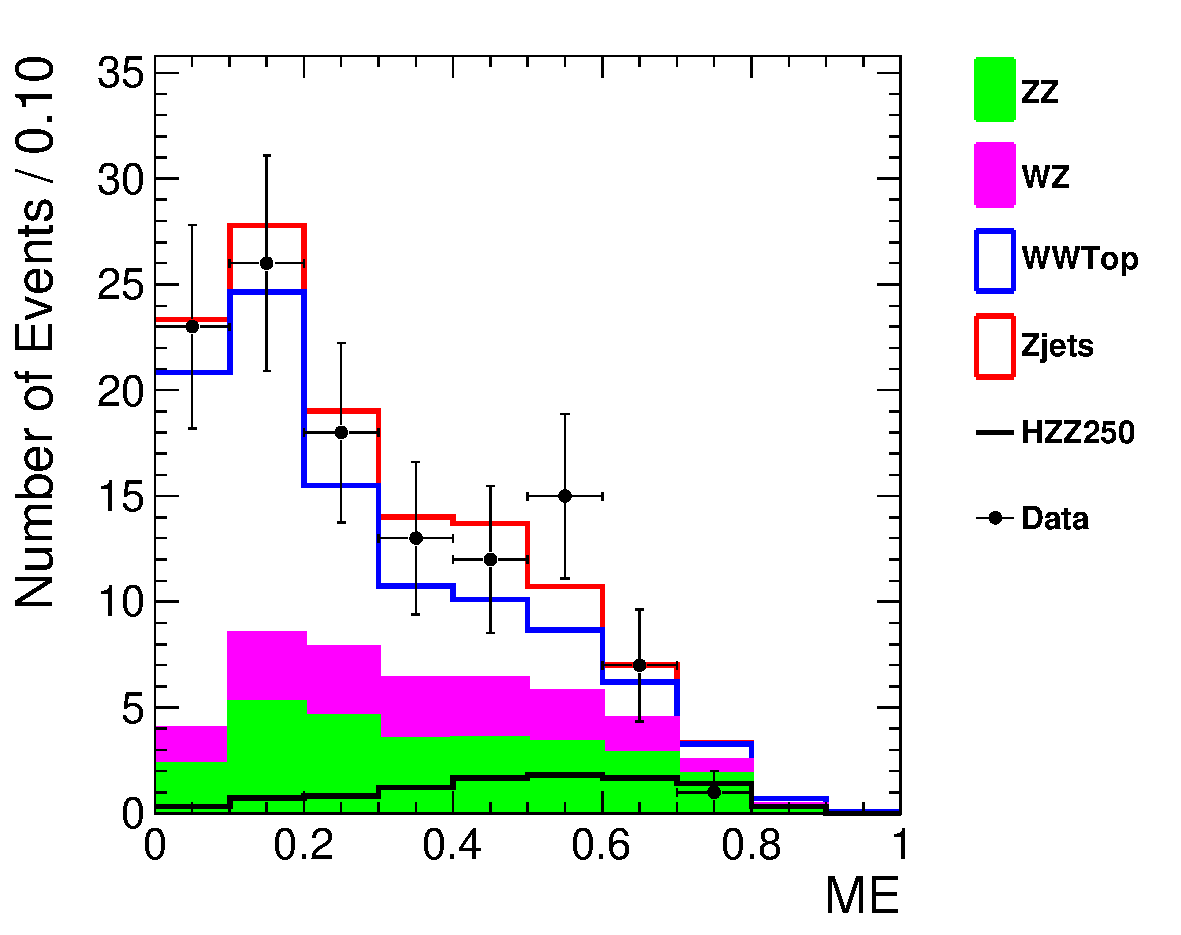
\includegraphics[width=0.4\textwidth,angle=0]{figures/ME_mH250_ee_stack_lin.pdf}} 
   \subfigure[]{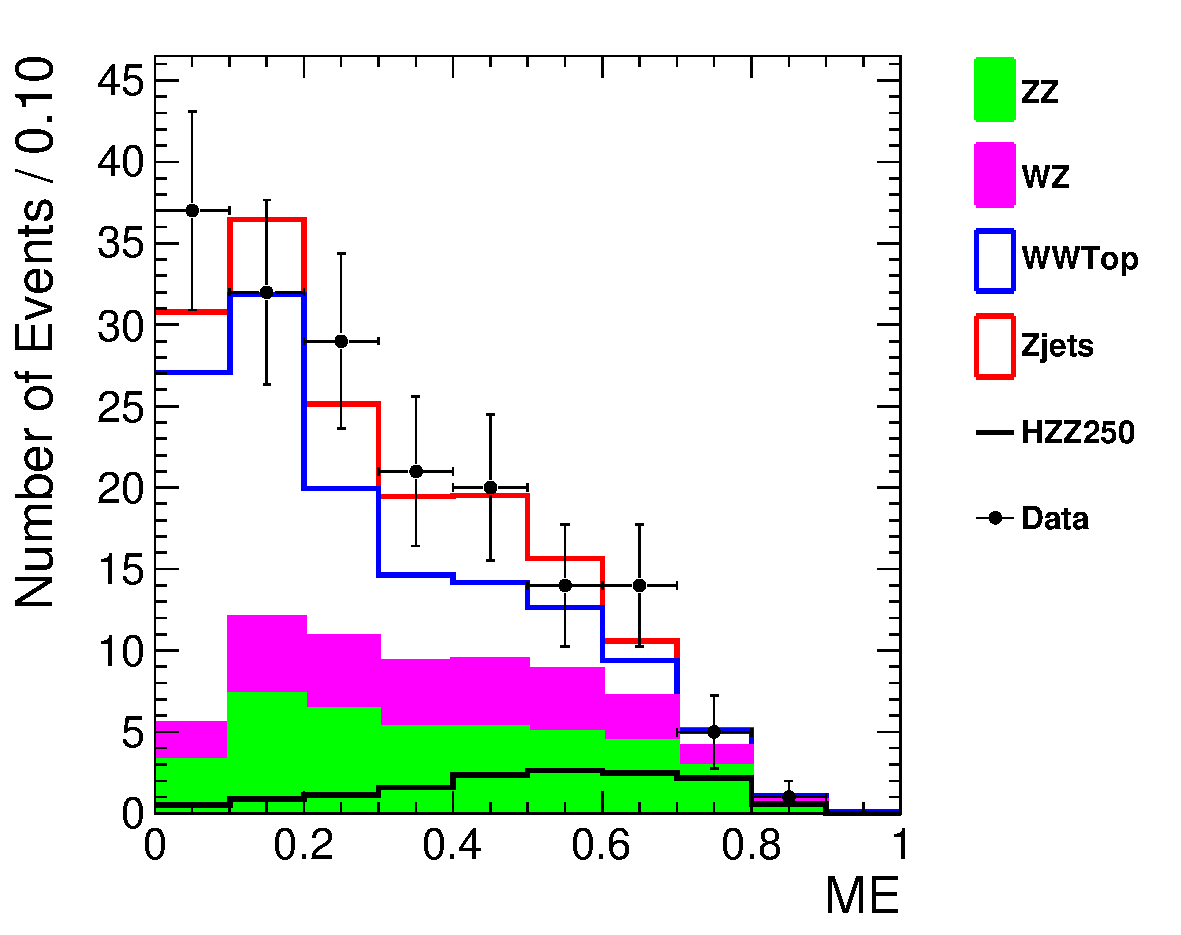
\includegraphics[width=0.4\textwidth,angle=0]{figures/ME_mH250_mm_stack_lin.pdf}} \\ 
   \caption{The matrix element output distribution for Higgs signal and background events 
for \mHi=250 $\GeVcc$ in ee (a) and $\mu\mu$ final state (b) after the higgs dependent selections. 
The distributions are normalized to \intlumi with the background scaled by the data-to-mc ratios derived from data.}
   \label{fig:histo_me_250_5fb}
\end{center}
\end{figure}

\begin{figure}[!ht]
\begin{center}
   \subfigure[]{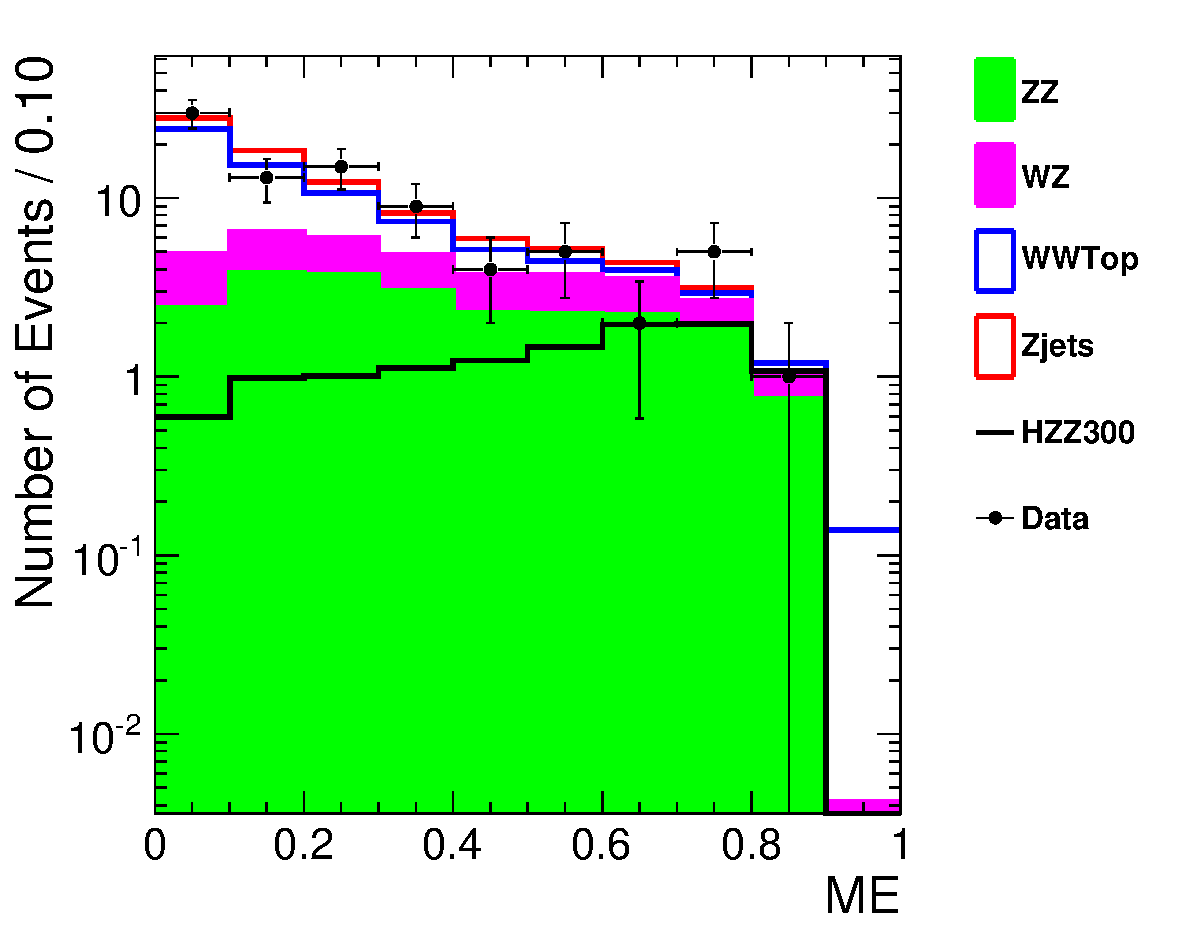
\includegraphics[width=0.4\textwidth,angle=0]{figures/ME_mH300_ee_stack_log.pdf}} 
   \subfigure[]{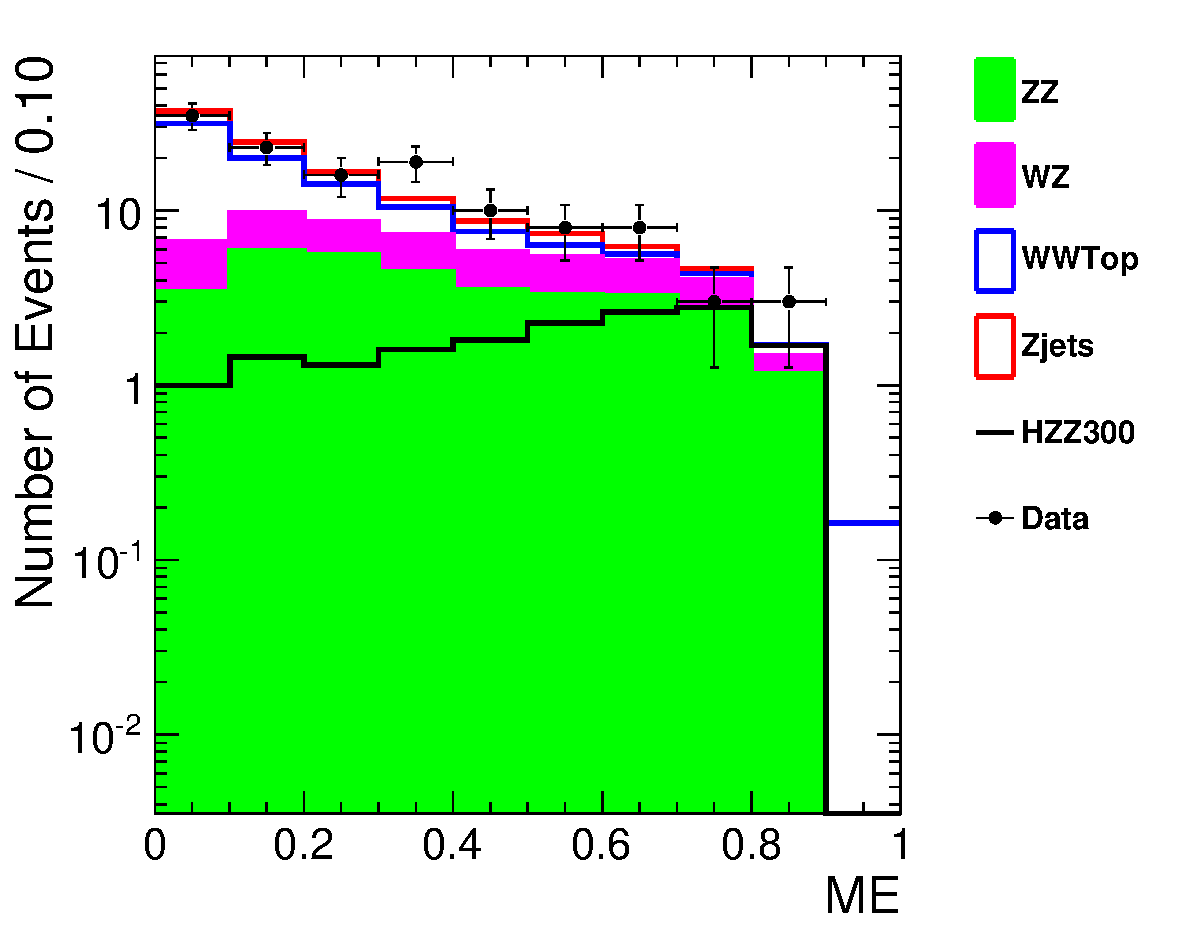
\includegraphics[width=0.4\textwidth,angle=0]{figures/ME_mH300_mm_stack_log.pdf}} \\ 
   \caption{The matrix element output distribution for Higgs signal and background events 
for \mHi=300 $\GeVcc$ in ee (a) and $\mu\mu$ final state (b) after the higgs dependent selections. 
The distributions are normalized to \intlumi with the background scaled by the data-to-mc ratios derived from data.}
   \label{fig:histo_me_300_5fb}
\end{center}
\end{figure}

\begin{figure}[!ht]
\begin{center}
   \subfigure[]{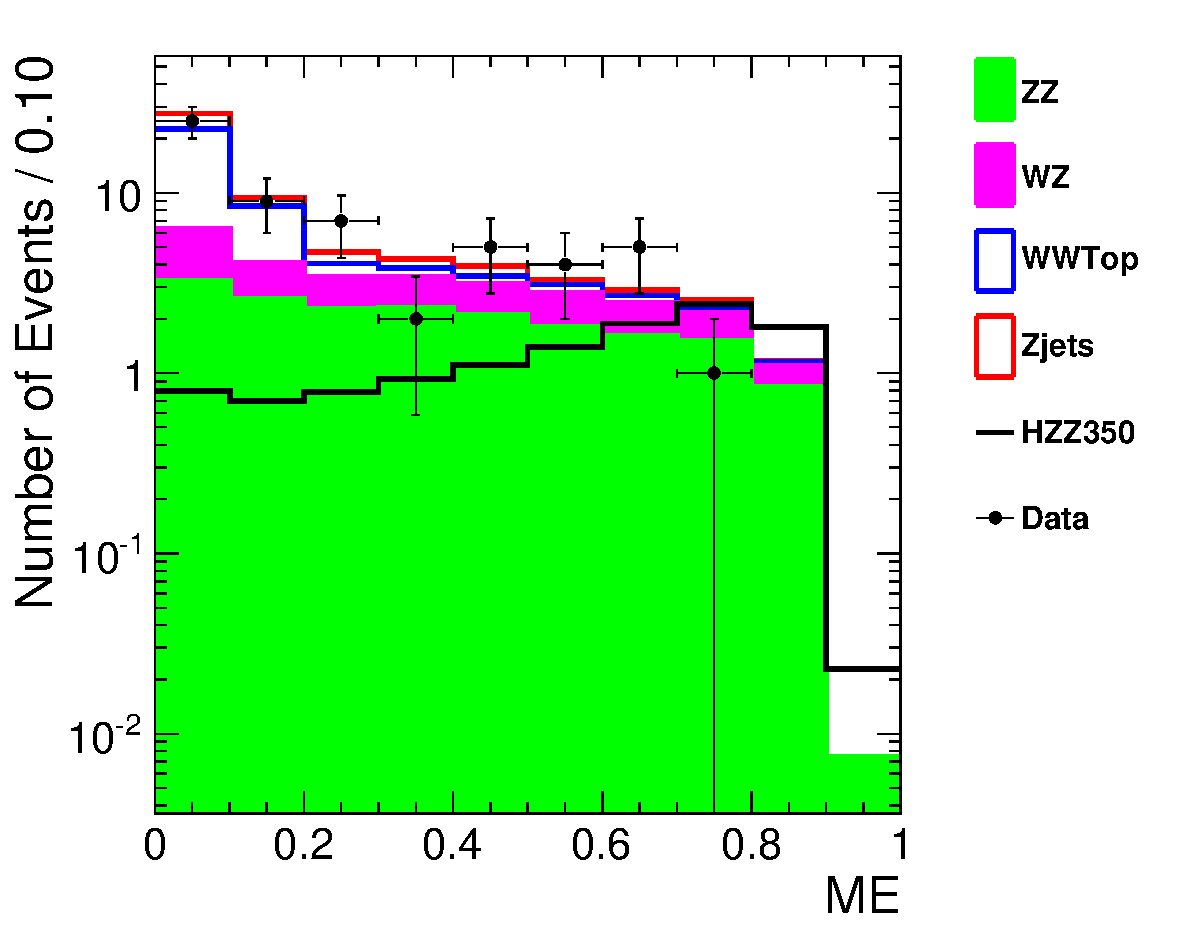
\includegraphics[width=0.4\textwidth,angle=0]{figures/ME_mH350_ee_stack_log.pdf}} 
   \subfigure[]{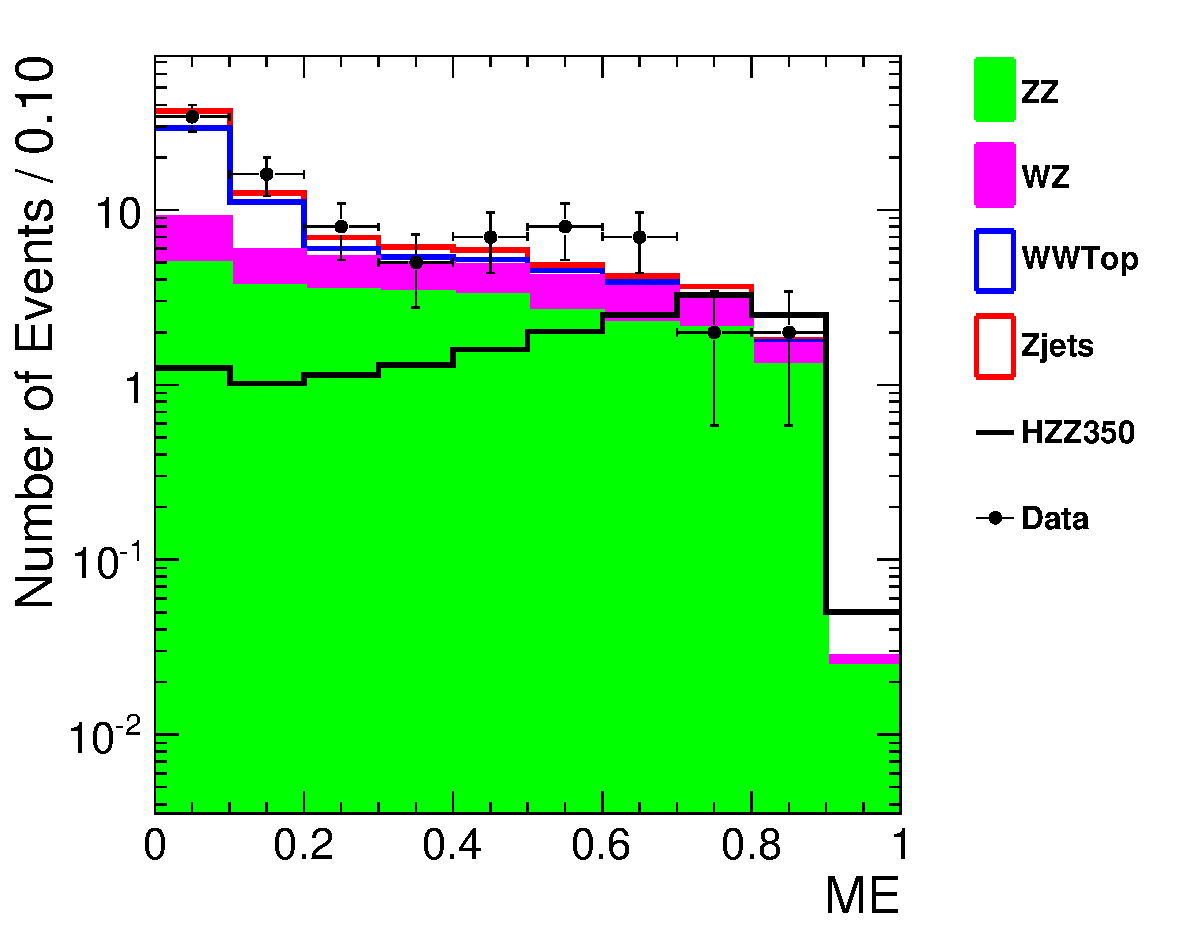
\includegraphics[width=0.4\textwidth,angle=0]{figures/ME_mH350_mm_stack_log.pdf}} \\ 
   \caption{The matrix element output distribution for Higgs signal and background events 
for \mHi=350 $\GeVcc$ in ee (a) and $\mu\mu$ final state (b) after the higgs dependent selections. 
The distributions are normalized to \intlumi with the background scaled by the data-to-mc ratios derived from data.}
   \label{fig:histo_me_350_5fb}
\end{center}
\end{figure}

\begin{figure}[!ht]
\begin{center}
   \subfigure[]{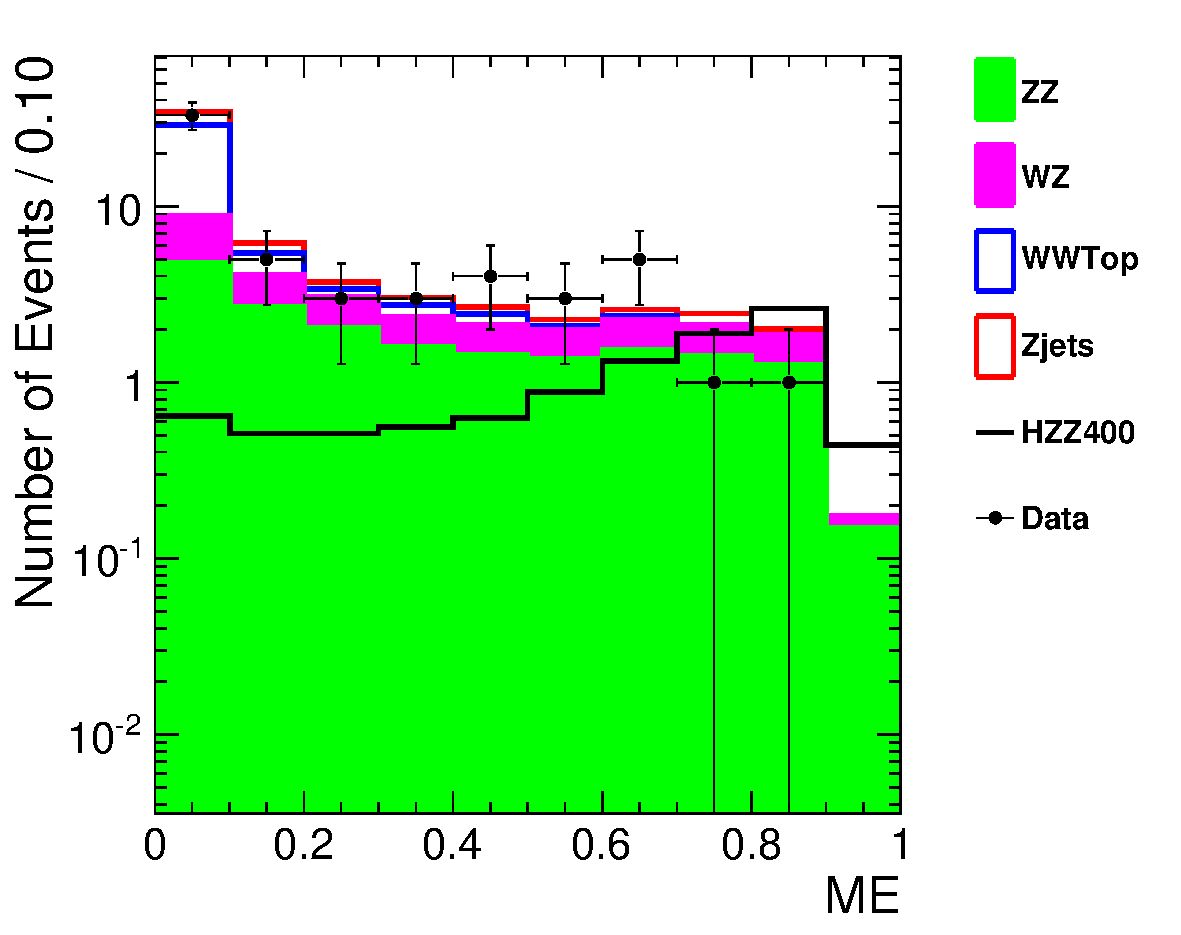
\includegraphics[width=0.4\textwidth,angle=0]{figures/ME_mH400_ee_stack_log.pdf}} 
   \subfigure[]{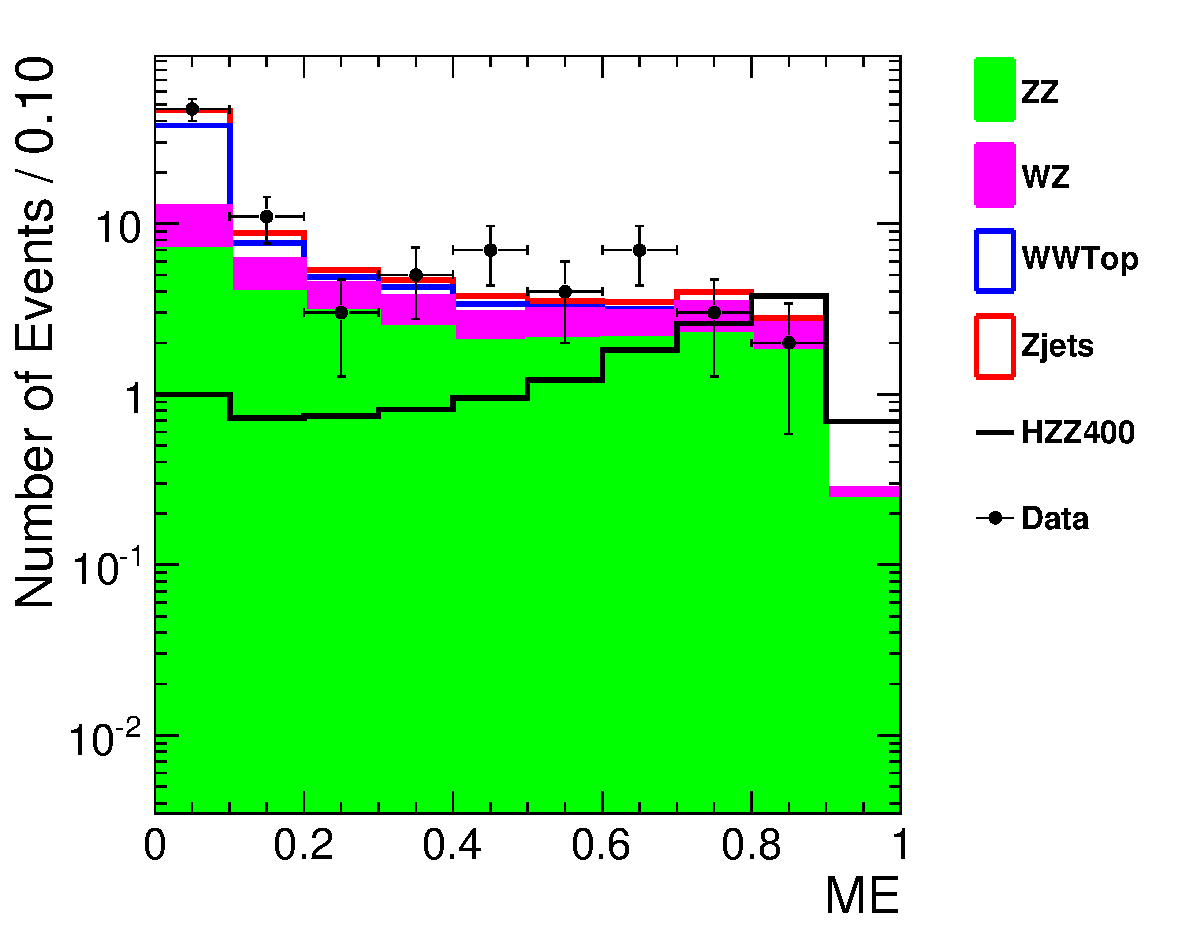
\includegraphics[width=0.4\textwidth,angle=0]{figures/ME_mH400_mm_stack_log.pdf}} \\ 
   \caption{The matrix element output distribution for Higgs signal and background events 
for \mHi=400 $\GeVcc$ in ee (a) and $\mu\mu$ final state (b) after the higgs dependent selections. 
The distributions are normalized to \intlumi with the background scaled by the data-to-mc ratios derived from data.}
   \label{fig:histo_me_400_5fb}
\end{center}
\end{figure}


\begin{figure}[!ht]
\begin{center}
   \subfigure[]{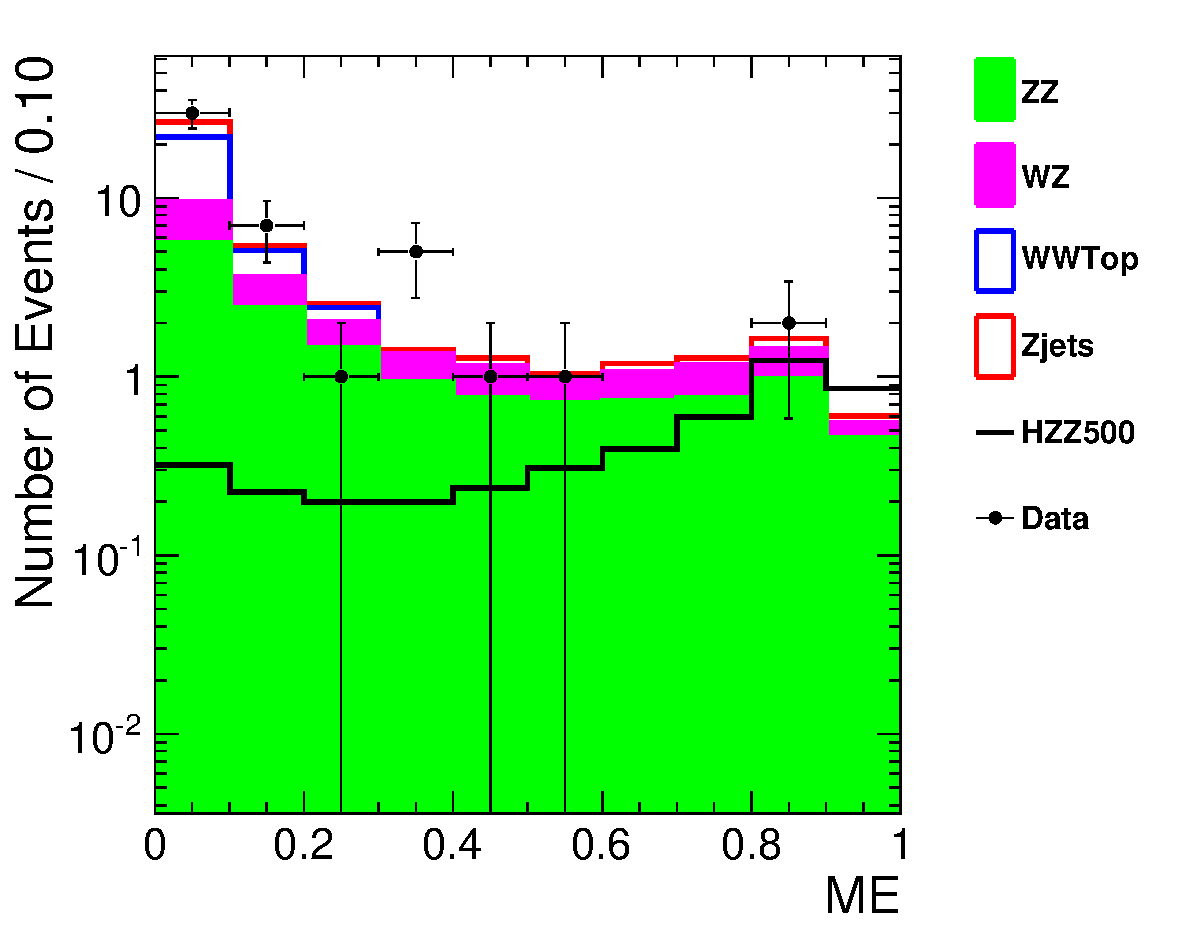
\includegraphics[width=0.4\textwidth,angle=0]{figures/ME_mH500_ee_stack_log.pdf}} 
   \subfigure[]{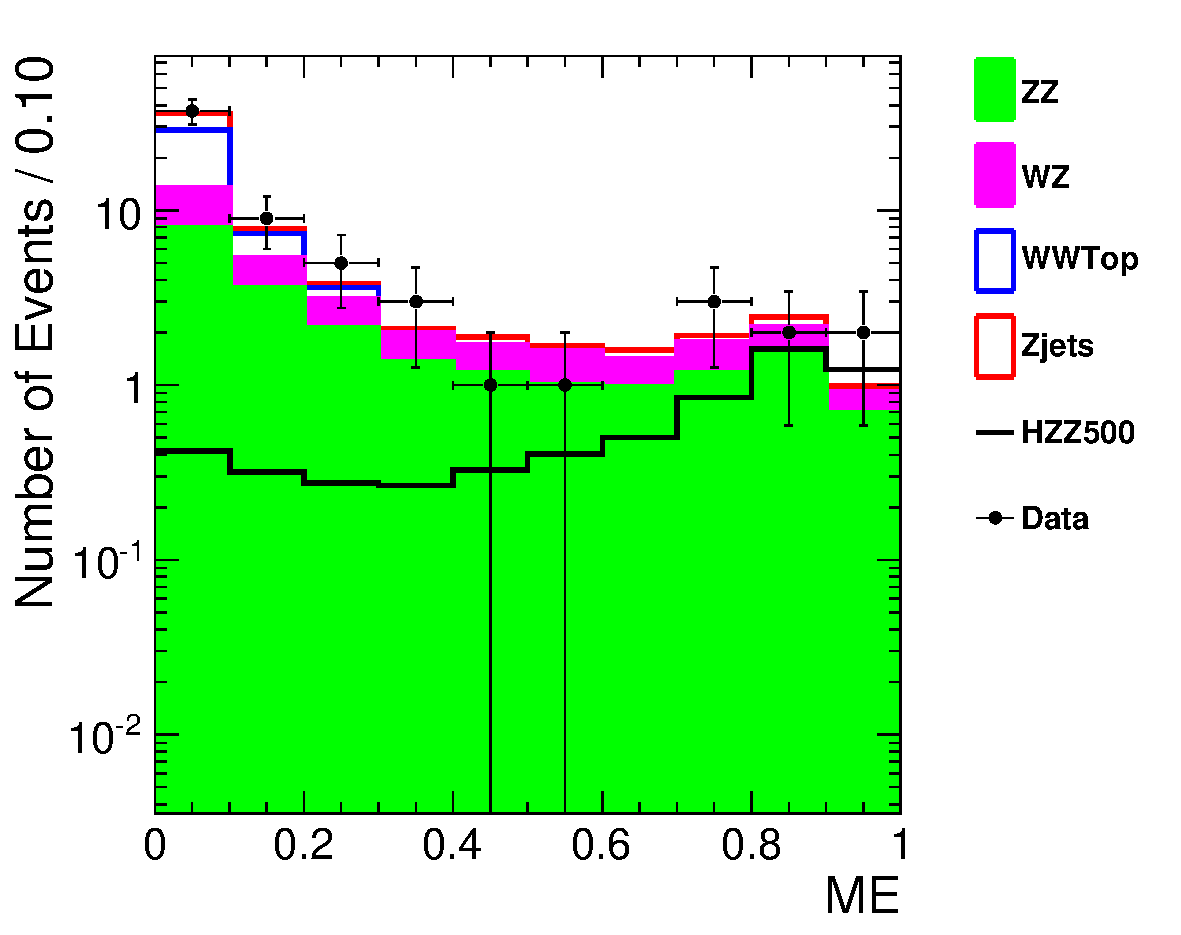
\includegraphics[width=0.4\textwidth,angle=0]{figures/ME_mH500_mm_stack_log.pdf}} \\ 
   \caption{The matrix element output distribution for Higgs signal and background events 
for \mHi=500 $\GeVcc$ in ee (a) and $\mu\mu$ final state (b) after the higgs dependent selections. 
The distributions are normalized to \intlumi with the background scaled by the data-to-mc ratios derived from data.}
   \label{fig:histo_me_500_5fb}
\end{center}
\end{figure}

\begin{figure}[!ht]
\begin{center}
   \subfigure[]{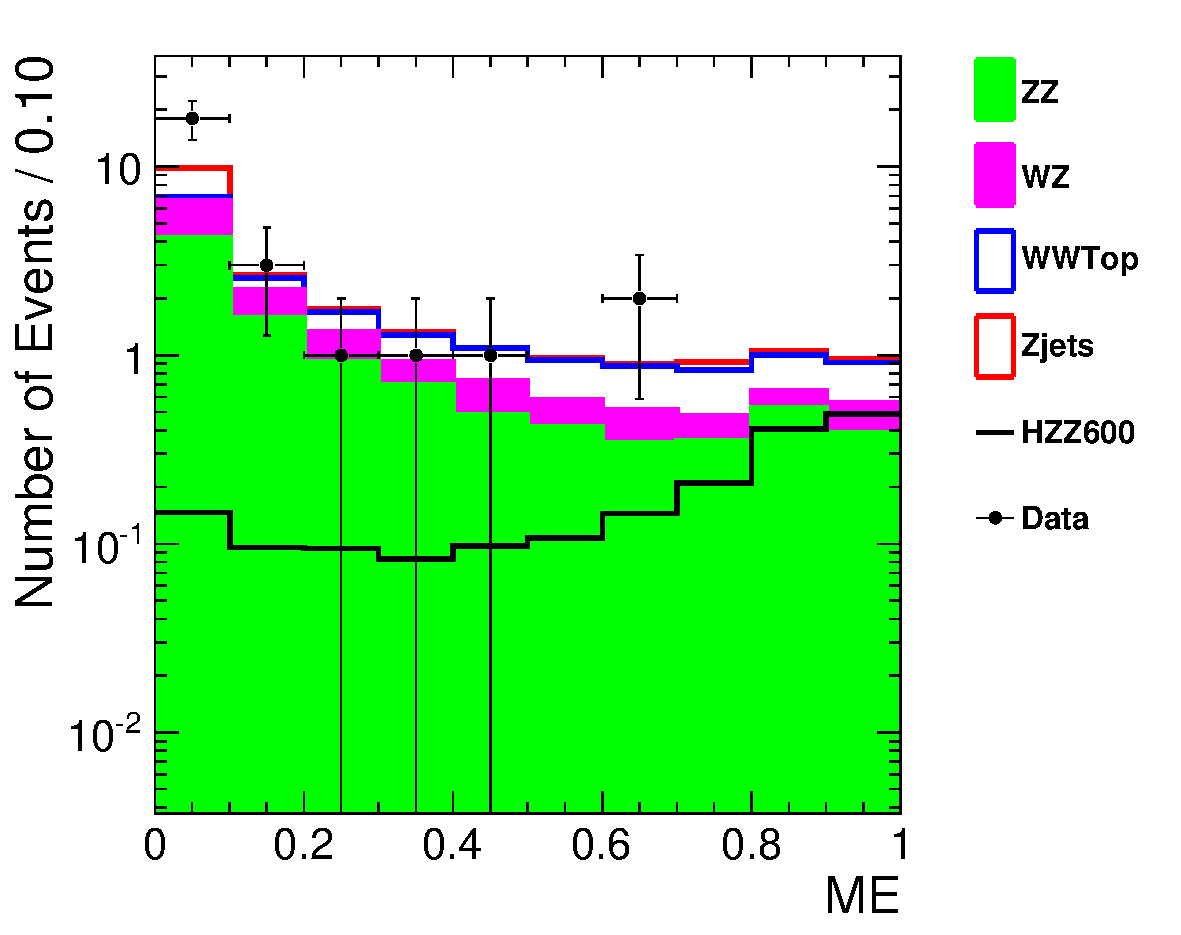
\includegraphics[width=0.4\textwidth,angle=0]{figures/ME_mH600_ee_stack_log.pdf}} 
   \subfigure[]{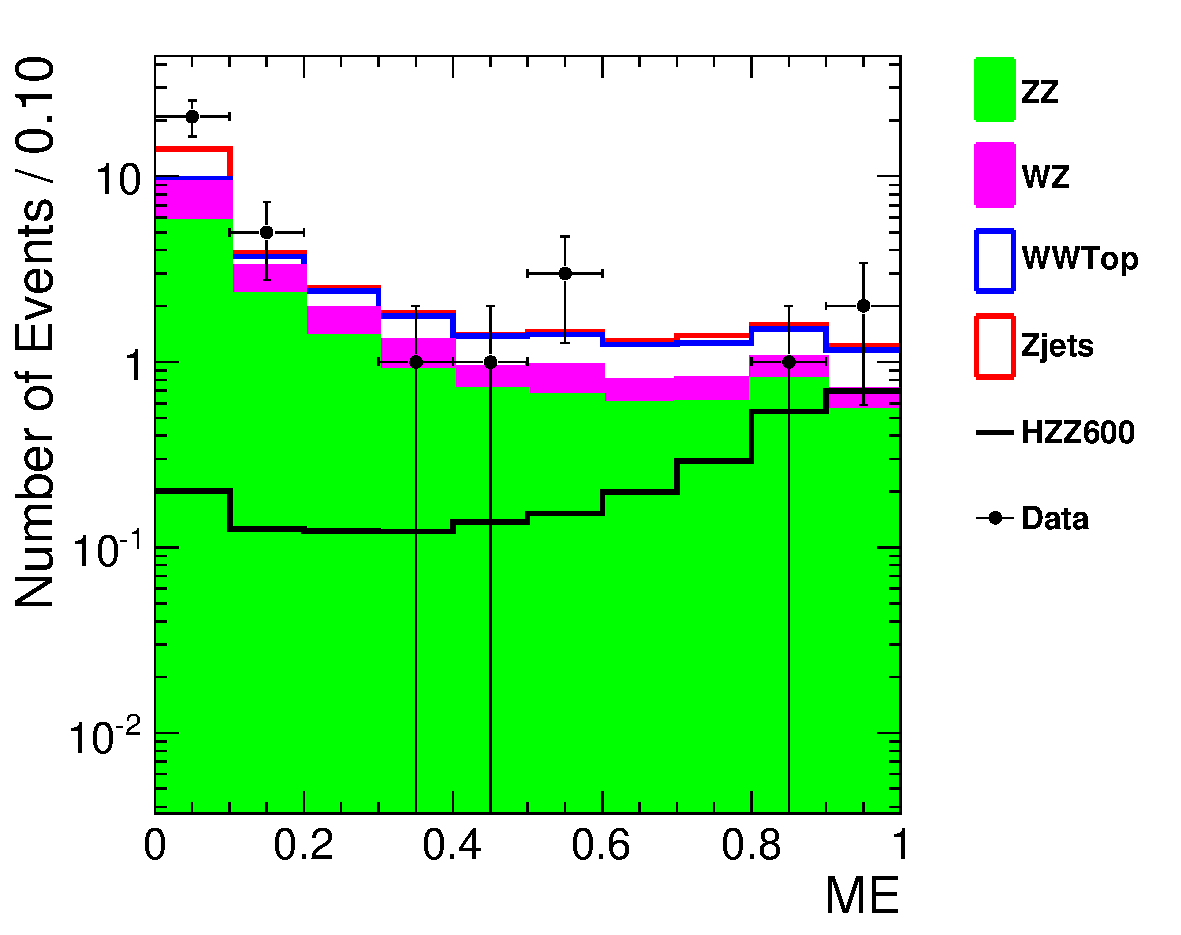
\includegraphics[width=0.4\textwidth,angle=0]{figures/ME_mH600_mm_stack_log.pdf}} \\ 
   \caption{The matrix element output distribution for Higgs signal and background events 
for \mHi=600 $\GeVcc$ in ee (a) and $\mu\mu$ final state (b) after the higgs dependent selections. 
The distributions are normalized to \intlumi with the background scaled by the data-to-mc ratios derived from data.}
   \label{fig:histo_me_600_5fb}
\end{center}
\end{figure}
%%%%%%%%%%%%%%%%%%%%%%




%%%%%%%%%%%%%%%%%%%%%%%%%%%%%%%
\begin{table}[!htbp]
\begin{center}
\begin{tabular}{ccccc}
\hline\hline
Mass & Observed & Median Expected & [-$\sigma$, +$\sigma$] & [-2$\sigma$, +2$\sigma$]\\\hline
\hline
\multicolumn{5}{c} {Cut-based Analysis} \\ 
\hline
250 & 1.62 & 1.62 & [1.17, 2.24] & [0.88, 2.98] \\
300 & 0.95 & 1.04 & [0.75, 1.44] & [0.56, 1.91] \\
350 & 0.60 & 0.68 & [0.49, 0.94] & [0.37, 1.25] \\
400 & 0.59 & 0.65 & [0.47, 0.91] & [0.35, 1.21] \\
500 & 1.61 & 1.19 & [0.86, 1.66] & [0.65, 2.20] \\
600 & 2.20 & 2.36 & [1.70, 3.28] & [1.28, 4.36] \\
\hline
\multicolumn{5}{c} {Shape Analysis Based on $M_T$} \\ 
\hline
250 & 1.50 & 1.38 & [1.00, 1.92] & [0.75, 2.56] \\
300 & 0.66 & 0.93 & [0.67, 1.29] & [0.51, 1.72] \\
350 & 0.55 & 0.63 & [0.45, 0.87] & [0.34, 1.16] \\
400 & 0.54 & 0.63 & [0.46, 0.88] & [0.34, 1.17] \\
500 & 1.58 & 1.08 & [0.78, 1.50] & [0.58, 1.99] \\
600 & 2.41 & 2.23 & [1.61, 3.10] & [1.21, 4.12] \\
\hline
\multicolumn{5}{c} {Shape Analysis Based on Matrix Element Output} \\ 
\hline
250 & 1.20 & 1.31 & [0.95, 1.83] & [0.71, 2.43] \\
300 & 0.99 & 0.87 & [0.63, 1.21] & [0.47, 1.60] \\
350 & 0.63 & 0.64 & [0.46, 0.88] & [0.35, 1.18] \\
400 & 0.56 & 0.64 & [0.46, 0.89] & [0.35, 1.19] \\
500 & 0.99 & 1.13 & [0.82, 1.57] & [0.61, 2.09] \\
600 & 1.96 & 2.43 & [1.75, 3.37] & [1.32, 4.48] \\
\hline\hline
\end{tabular}
\end{center}
\caption{The observed and expected cross section ratio limits as a function 
of the Higgs mass, together with the 1/2-$\sigma$ uncertainty bands obtained in the cut-and-count analysis 
and shape analyses based on both $M_T$ variable and matrix element output.
The limits correspond to an integrated luminosity of \intlumi, shown in Figure~\ref{fig:limits_5fb}.}
\label{tab:limits_5fb}
\end{table}
%%%%%%%%%%%%%%%%%%%%%%%%%%%%%



%%%%%%%%%%%%%%%%%%%%%%%%%%%%%
\begin{figure}[!htbp]
  \begin{center}
  \subfigure[Cut-based Analysis]{
  \label{subfig:cutbased}
  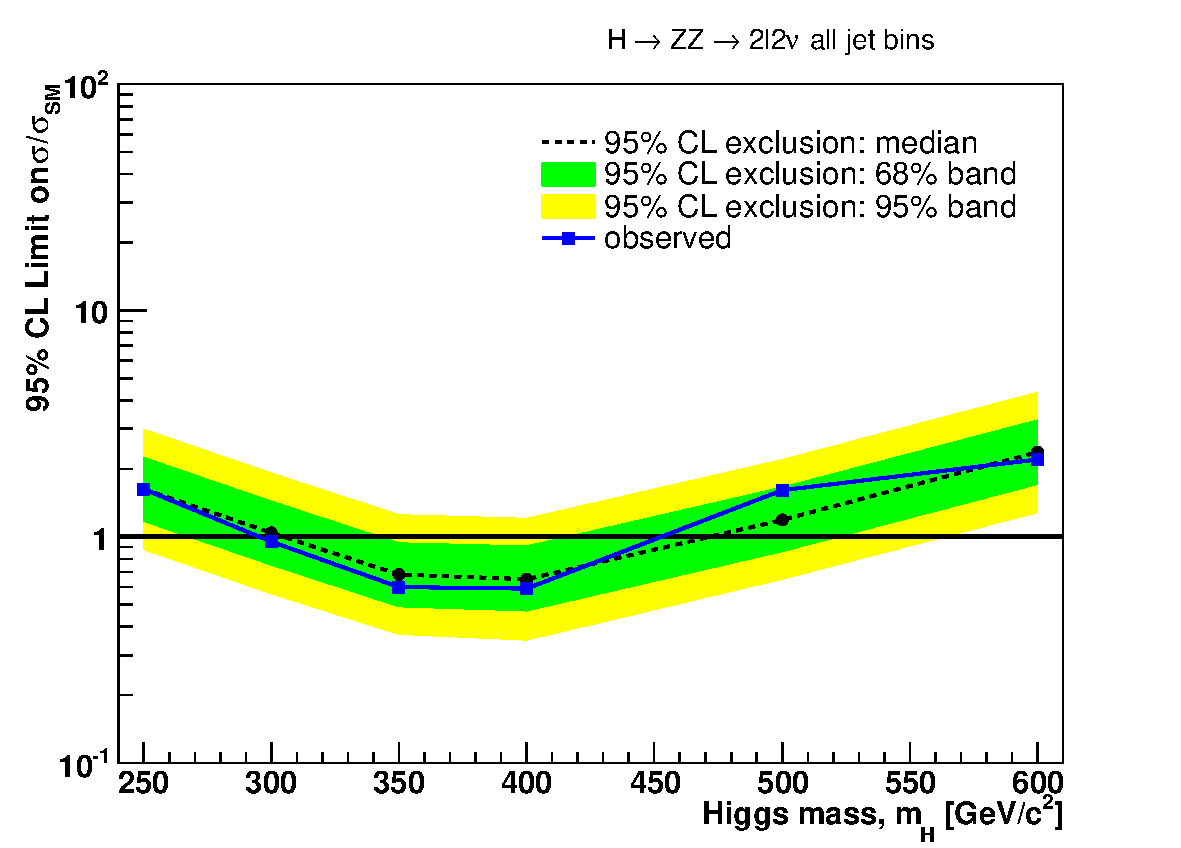
\includegraphics[width=0.5\textwidth]{figures/limits_cut_5fb.pdf}} \\
\end{center}
  \subfigure[$M_T$ Shape Analysis]{
  \centering
  \label{subfig:mtshape}
   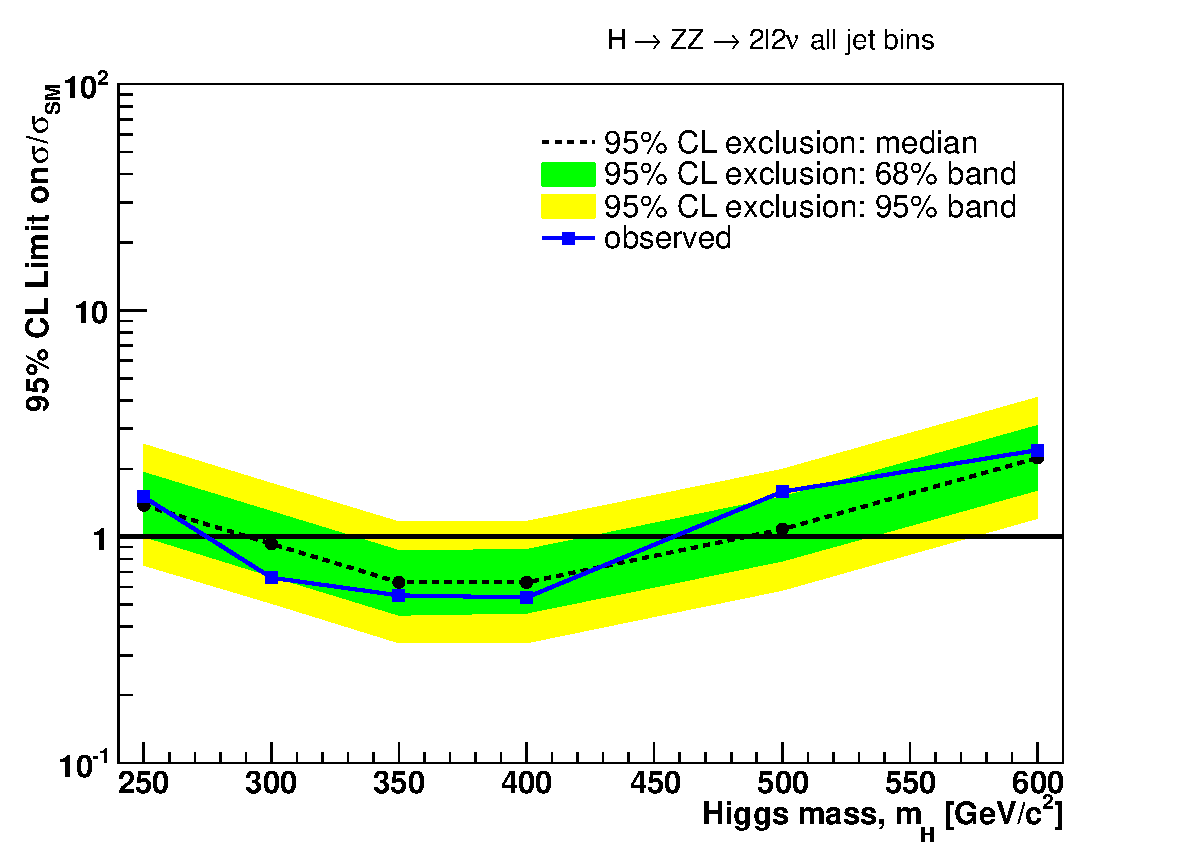
\includegraphics[width=0.5\textwidth]{figures/limits_mtshape_5fb.pdf}}
  \subfigure[Matrix Element Shape Analysis]{
  \centering
  \label{subfig:meshape}
   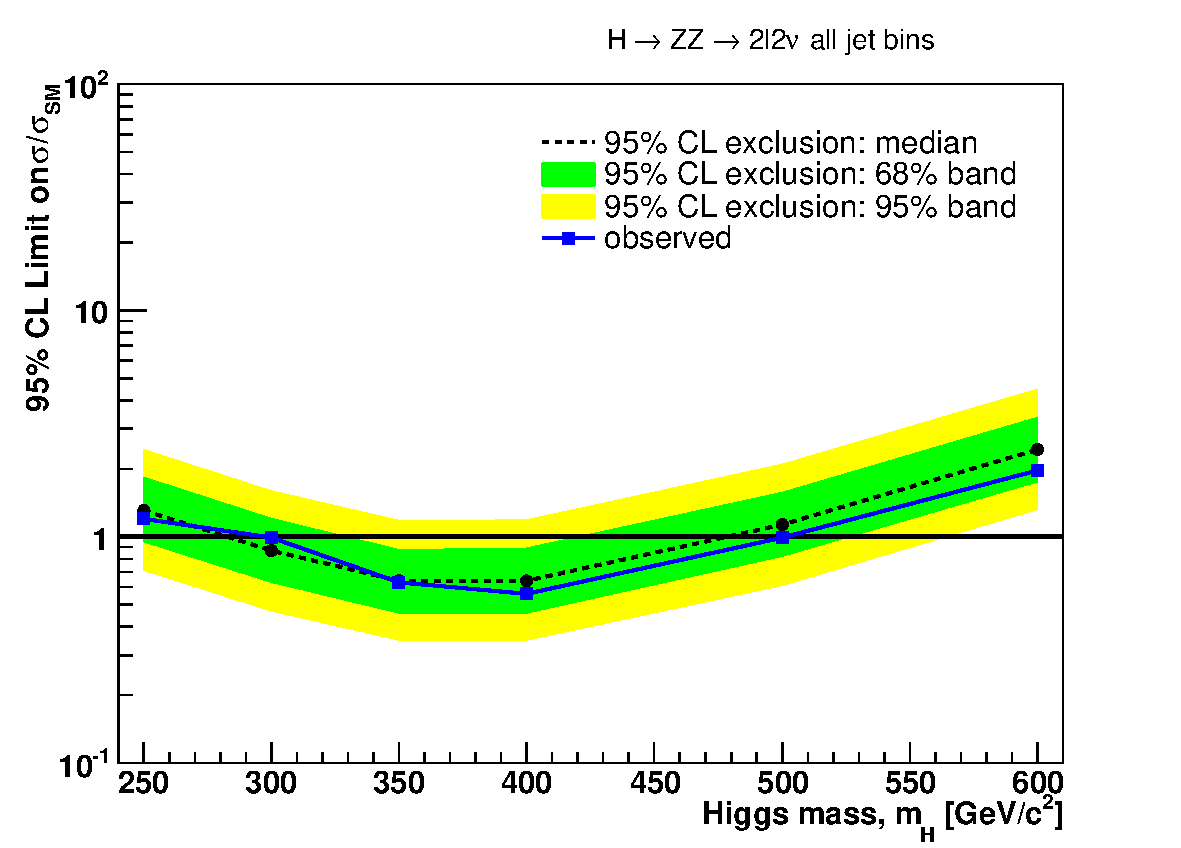
\includegraphics[width=0.5\textwidth]{figures/limits_meshape_5fb.pdf}}
\caption{The observed and expected upper limits at 95\% C.L. for \intlumi\ of data for the 
	cut-based analysis \subref{subfig:cutbased} and 
	shape analyses based on both $M_T$ variable \subref{subfig:mtshape} 
	and matrix element output \subref{subfig:meshape} The values are 
	tabulated in Table~\ref{tab:limits_5fb}.  
}	
\label{fig:limits_5fb}
\end{figure}
%%%%%%%%%%%%%%%%%%%%%%%%%%%%%
